\documentclass[a4paper]{article}

\usepackage{a4wide}
\usepackage{graphicx}

\author{Bram Pulles}
\title{\textbf{bTCP: basic Transmission Control Protocol}}

\begin{document}
\maketitle

\tableofcontents
\pagebreak

\section{Finite state machines}
This section describes all of the finite state machines for bTCP. In every finite state machine figure, the transitions where messages are received or send have the part being received on top and the part being send underneath. Further, a - indicates that nothing is send/received. At last, everything before the vertical bar indicates the flags which are set and everything after the bar is the content/values of the segment.

The FSMs are divided into three categories: connection establishment, sending/receiving data and connection termination. This is done so a concise FSM can be shown for every state providing better readability. Note that the \texttt{ESTABLISHED}, \texttt{SEND} and \texttt{RECV} states connect the different FSMs.

	\subsection{Connection establishment}
	The finite state machines for the establishment of a connection can be seen in figure \ref{fig: phase 1 client} and \ref{fig: phase 1 server}, for the client and server respectively. Note that the client cannot verify if the server actually received the ACK. This can result in a state where the client thinks it is connected while the server thinks it is not. To circumvent this problem the server also goes to the connected state if it receives another message from the client than the ACK. This works because if the server receives another message that means that the client thinks it is connected and thus received the message from the server. The data which is send by the client works as an ACK. The data is not saved, but will be resend by the client later anyways. This way the three way handshake will always succeed, also if segments are lost, in particular the last ACK send from the client.
	\begin{figure}[h]
		\centering
		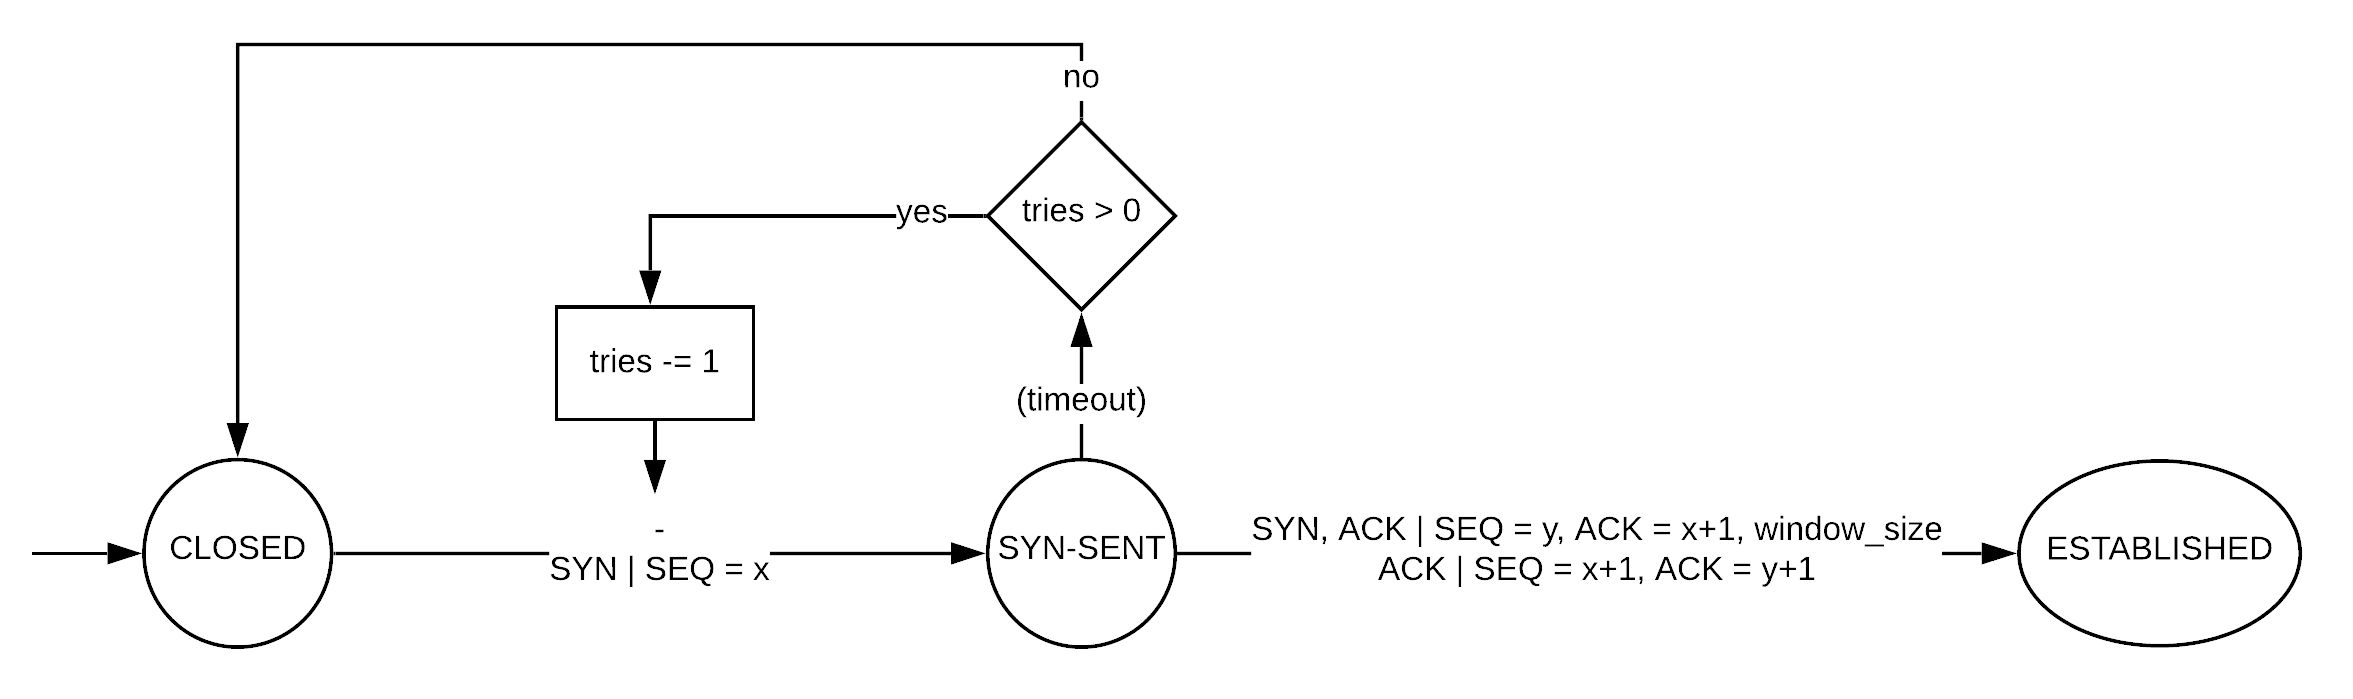
\includegraphics[width = \textwidth]{phase1_client.png}
		\caption{FSM connection establishment client.}
		\label{fig: phase 1 client}
	\end{figure}
	\begin{figure}[h]
		\centering
		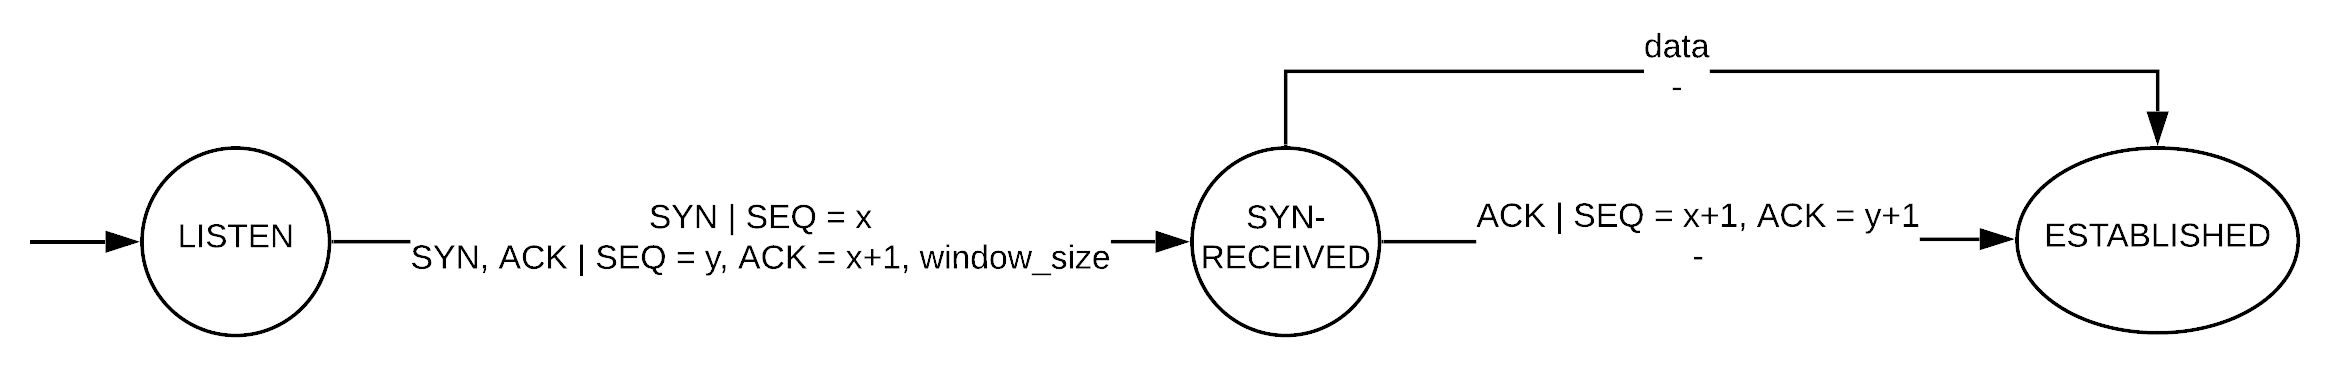
\includegraphics[width = \textwidth]{phase1_server.png}
		\caption{FSM connection establishment server.}
		\label{fig: phase 1 server}
	\end{figure}

	\subsection{Sending/receiving data}
	The finite state machines for an established connection where data is being send can be seen in figure \ref{fig: phase 2 client} and \ref{fig: phase 2 server}, for the client and the server respectively. The FSM for the server is extremely simply, since it only sends back ACKs for segments it received, that is all. The FSM for the client is a little more difficult. I had a bit of trouble with displaying the actions in the FSM, so it will just provide a basic abstract overview. See the other sections, in particular the one on reliability and the one on flow control, for more information.
	\begin{figure}[h]
		\centering
		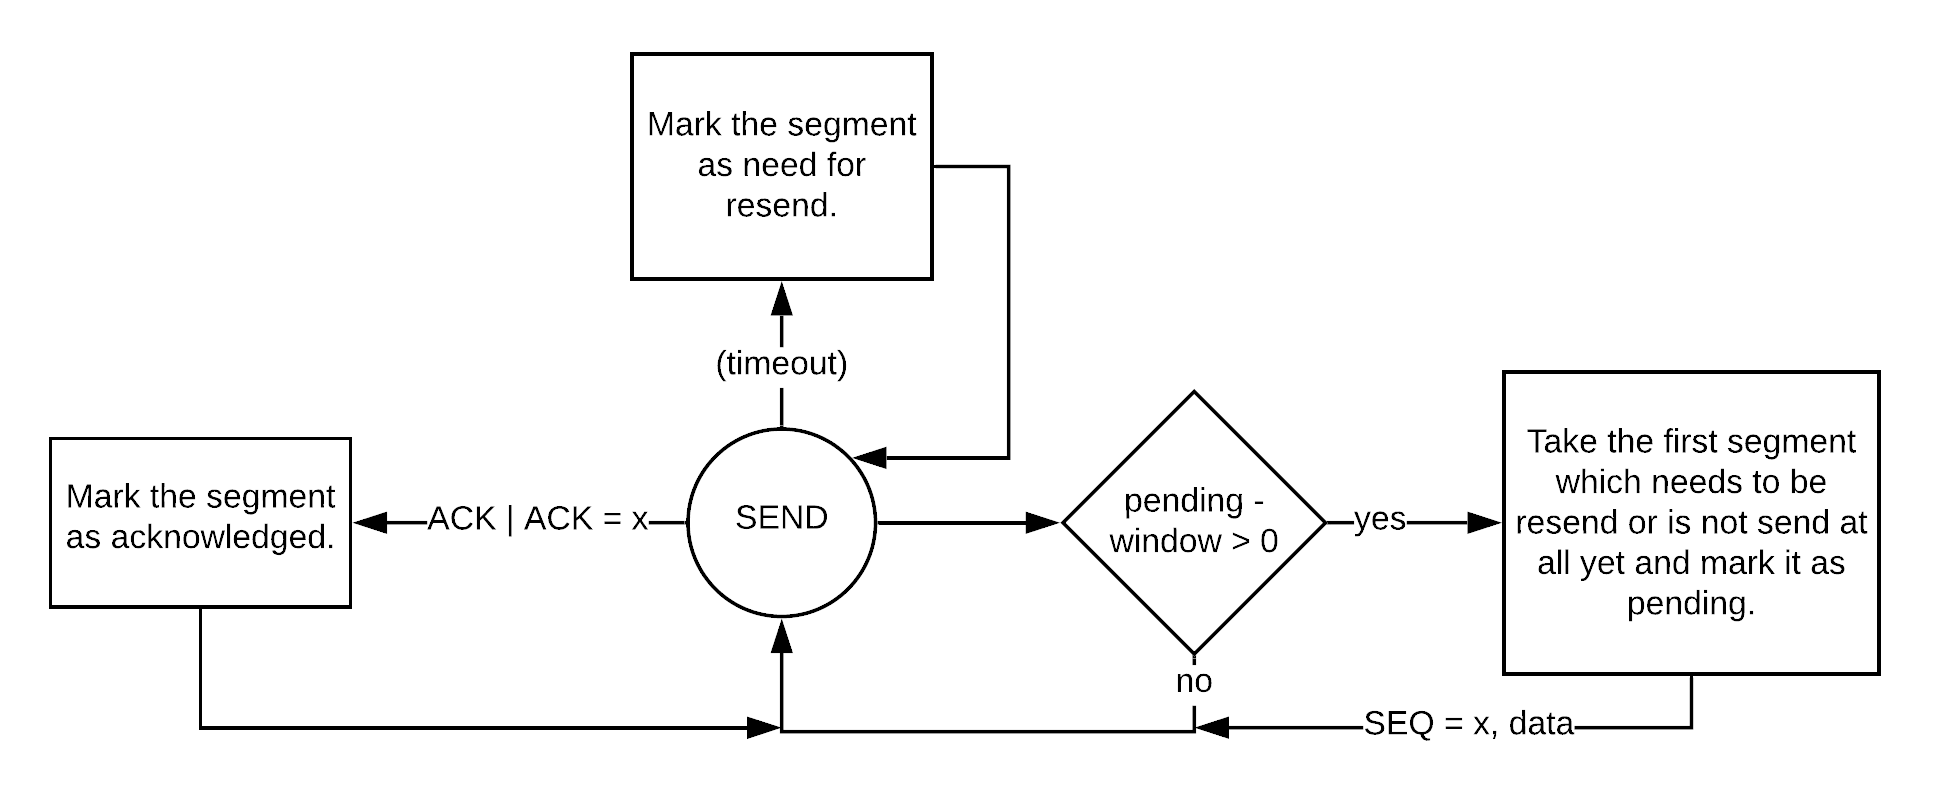
\includegraphics[width = \textwidth]{phase2_client.png}
		\caption{FSM sending data client.}
		\label{fig: phase 2 client}
	\end{figure}
	\begin{figure}[h]
		\centering
		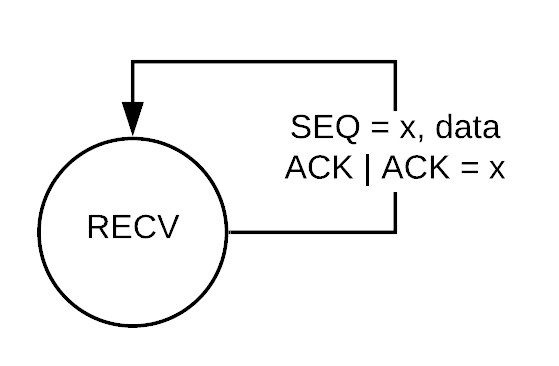
\includegraphics[width = .3\textwidth]{phase2_server.png}
		\caption{FSM receiving data server.}
		\label{fig: phase 2 server}
	\end{figure}

	\subsection{Connection termination}
	The finite state machines for the termination of a connection can be seen in figure \ref{fig: phase 3 client} and \ref{fig: phase 3 server}, for the client and server respectively. Note that the server does not verify if the ACK send is received by the client. However, since the client terminates the connection after having done a certain amount of tries (each with a timeout), it does not matter since both will close correctly anyways.
	\begin{figure}[h]
		\centering
		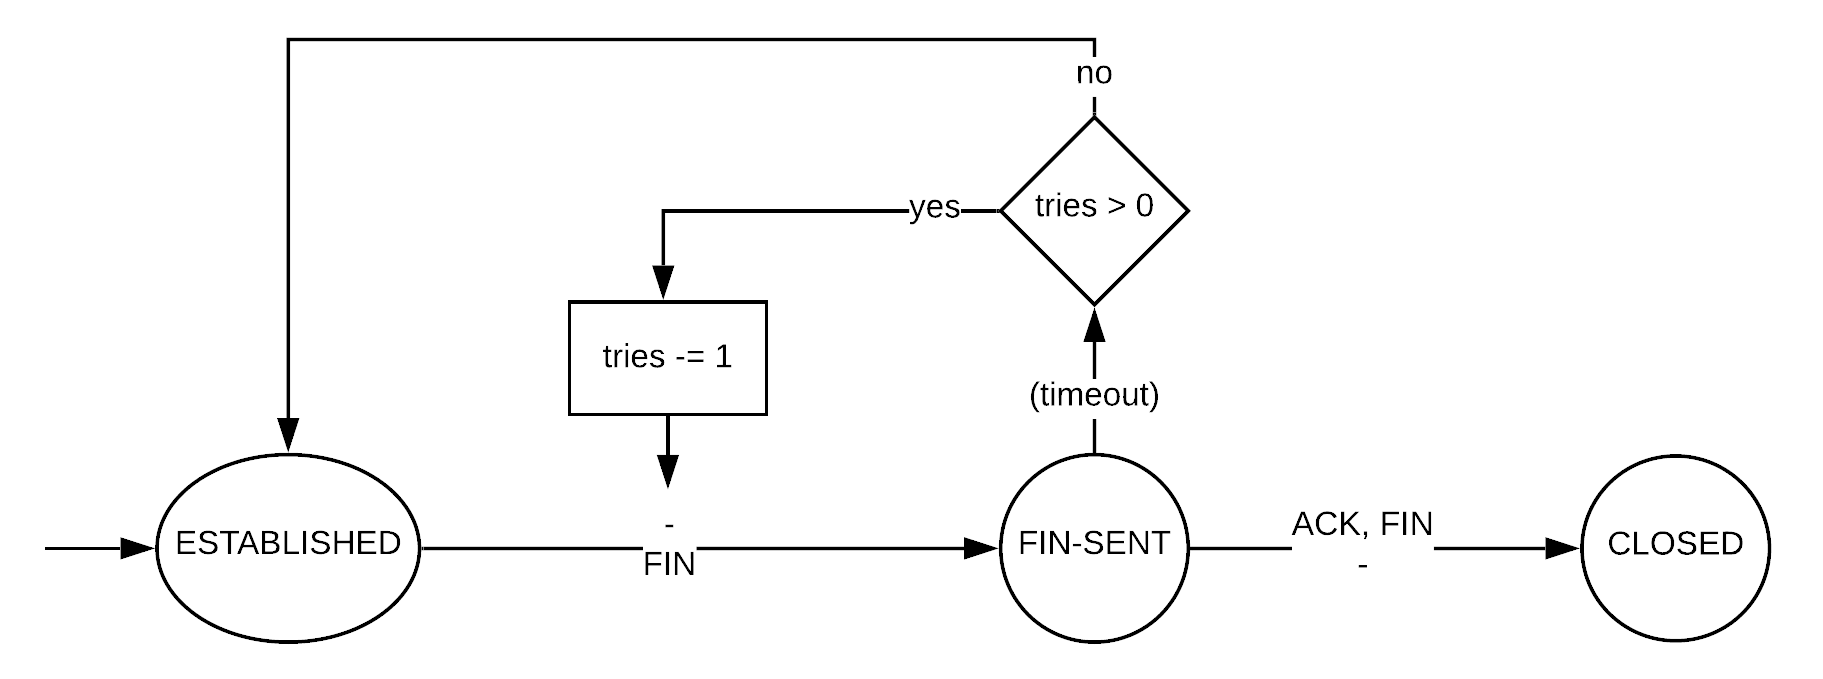
\includegraphics[width = \textwidth]{phase3_client.png}
		\caption{FSM connection termination client.}
		\label{fig: phase 3 client}
	\end{figure}
	\begin{figure}[h]
		\centering
		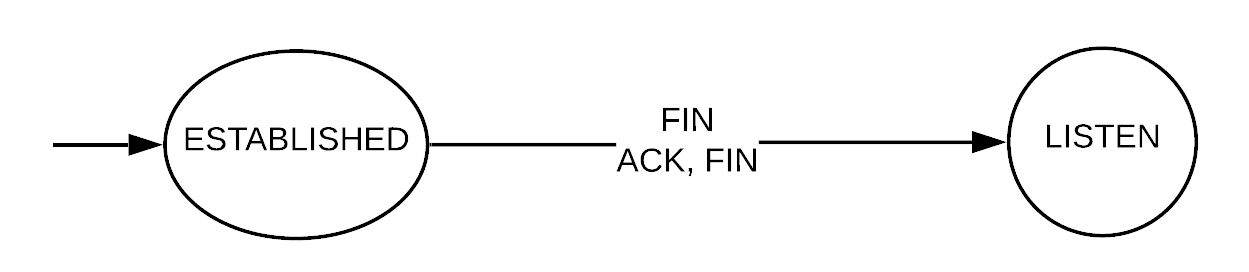
\includegraphics[width = .7\textwidth]{phase3_server.png}
		\caption{FSM connection termination server.}
		\label{fig: phase 3 server}
	\end{figure}

\section{Reliability}
Reliability is provided by an implementation of Selective Repeat (SR). SR is chosen over Go~Back~N, because SR is more efficient when the window size is relatively big (this decision was made before the discovery of the window size limit, see section \ref{sec: window size}). Further it was chosen because the multiple logical timers can be implemented by using one hardware timer, which is also done in the implementation.

\section{Flow control}
Flow control is implemented in the same way as it is in TCP. So we have a list with pending segments, i.e. segments which are send but not yet acknowledged. We also have a window size which we receive from the server with every ACK that is send and is calculated by the size of the buffer minus the number of segments in the buffer. Every time the client wants to send a segment to the server it first checks if the number of segments in the pending list is smaller than the current window size of the server iff this is the case a segment is send. With every timeout the corresponding segment is removed from the pending list (and marked to be resend) since we assume that the segment is lost in the network. Note that this is one of the causes for the problem with the window size described in section \ref{sec: window size}, because the segment might not be lost but the server can have a too high workload instead.

\section{Implementation}
This section describes some design choices on the implementation level.

	\subsection{bTCP socket interface}
	The description of the bTCP protocol in the assignment tells us that we only need to have traffic being send from the client to the server. The server will only send ACKs back to the client for receiving its data. This means that we only need to think about the receiving window of the server. It also means that only the client needs to keep a timer in order to determine when to resend a packet.

	The template provided for this project does not account for this and gives a timeout and window size parameter to both the client and the server even though they both only need one. I refractored the bTCP socket interface so it does not need to be a class anymore containing these variables. This makes it easier to test the individual functions as well as providing a cleaner code base, since unnecessary variables are removed from both the client and the server.

	\subsection{Window size}\label{sec: window size}
	The implementation works the best with a low window size of about 30 and lower, this has to do with the load on the server. If the server says it has a bigger window size it would have to handle more segments in the same amount of time. However, the server is not fast enough to handle a lot of segments which will result in a timeout at the client side. When the client detects a timeout it assumes that the segment is lost and tries to send it again. This results in an even bigger workload on the server and even more timeouts. This will cause a buffer overflow as well as a lot of timeouts on the client side until the client just gives up. So depending on the performance of the server the window size can be adjusted. The timeout on the client can also be increased to give the server more time to process the segments. But practice learns that it is best just to give an accurate window size for the server.

	\subsection{Threads, locks and atomic operations}
	Both the server and the client use some threads and locks. The server spawns a lock for every incoming segment. These segments are added to a list which is processed by a dedicated thread which creates ACKs and sends these back to the client. The client has a dedicated thread for processing the received ACKs, sending data and running a timer. We only use one thread which runs a timer. By using the pending list which stores the time at which a segment was send we can calculate whether a timeout occurred by comparing this time send with the current time. This way only one hardware timer is needed for multiple logical timers.

	In order to keep all of the variables used by the client safe from running conditions mutex locks are used. Note that we also make use of the fact that some operations are atomic in Python, e.g. the \texttt{append()} and \texttt{pop()} function for list objects.

\end{document}
